\section{Fundamentos teóricos}
En esta sección se detallan los conceptos, familias de modelos y algoritmos necesarios para la elaboración del trabajo posterior. Se usarán los conocimientos aprendidos en las asignaturas de Aprendizaje Automático, Visión por Computador y Metaheurísticas además de las referencias indicadas en cada caso.


En la Sección \ref{sec:gd} aparecen los optimizadores basados en GD que se utilizarán en la experimentación: Adam, AdamW, NAG y RMSProp, mientras que en la Sección \ref{sec:mh} se hace lo propio con los algoritmos MH: SHADE y SHADE-ILS. Para finalizar, en la Sección \ref{sec:tests} se describen los tests estadísticos que más tarde se emplearán en la experimentación para un análisis riguroso de los rendimientos de los modelos.

\subsection{Redes neuronales y aprendizaje profundo}
\label{sec:profundo}

\subsubsection{Red neuronal}

Una red neuronal es un modelo computacional inspirado en la manera en la que las neuronas se conectan en el cerebro humano procesando la información. Consiste en capas interconectadas con nodos llamados neuronas, donde cada conexión tiene un peso asociado. Cada neurona normalmente aplica una función no linear, llamada función de activación, a la suma ponderada de las entradas de la capa anterior, permitiendo al modelo aprender relaciones complejas \cite{stanford_231}. Este tipo de redes se denominan totalmente conectadas. Sus componentes básicos son:

\begin{itemize}
	\item Capa de entrada: recibe la información.
	
	\item Capas ocultas: son las capas intermedias, que realizan los cálculos.
	
	\item Capa de salida: produce la salida del modelo.
\end{itemize}

El ejemplo más sencillo es el Perceptrón \cite{perceptron}, una red neuronal de una sola capa oculta y una sola neurona como podemos ver en la Figura \ref{fig:Perceptron}. Es un clasificador lineal, es decir, sólo puede resolver tareas cuyos datos sean linealmente separables. En su versión original su función de activación $f$ es la función signo. Para problemas más complejos que no sean lineales necesitamos usar redes neuronales con varias capas ocultas.


\begin{figure}
    \centering
    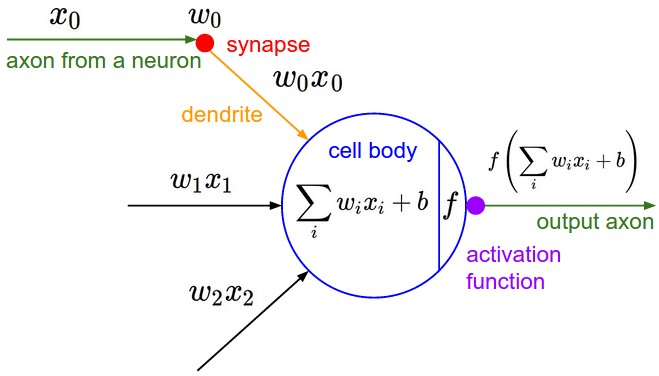
\includegraphics[width=0.75\linewidth]{Plantilla_TFG_latex//imagenes//Inf//2.Fund/neuron_model.jpeg}
    \caption[Representación esquemática de una neurona artificial inspirada en el modelo biológico]{Representación esquemática de una neurona artificial inspirada en el modelo biológico. La imagen ilustra la analogía entre una neurona biológica y una neurona artificial en una red neuronal. Las entradas $x_0,x_1,x_2$  representan señales provenientes de otras neuronas, con pesos sinápticos $w_0, w_1, w_2$ que modulan su importancia. En la biología, estas señales viajan a través del axón de una neurona y se transmiten mediante sinapsis (en rojo) a la dendrita (en naranja) de otra neurona. En la neurona artificial, las entradas ponderadas se combinan el cuerpo celular (en azul) mediante una suma ponderada $\sum_i w_ix_i + b$, donde $b$ es un sesgo. Esta combinación es procesada por una función de activación $f$ (en morado), cuya salida viaja a través del axón de salida (en verde), propagando la información a la siguiente capa de la red. Obtenida de \cite{stanford_231}.}
    \label{fig:Perceptron}
\end{figure}


\subsubsection{Aprendizaje profundo y redes neuronales profundas}

Las redes neuronales profundas tienen varias capas ocultas, generalmente más de dos. La profundidad de una red viene determinada por el número de capas ocultas que tiene, y ésta permite aprender representaciones jerárquicas de los datos, lo que habilita a las redes neuronales profundas a capturar patrones más complejos en los datos en comparación con redes con menos profundidad \cite{stanford_231}.

El aprendizaje profundo es una rama del aprendizaje automático que se centra en las redes neuronales profundas. Generalmente se usan modelos muy profundos con un alto número de parámetros y grandes cantidades de datos para resolver tareas complejas. Esto supone que se requiere de mucho poder computacional y de algoritmos avanzados para optimizar sus parámetros. Este tipo de modelos obtiene un gran rendimiento en tareas como el procesamiento del lenguaje natural, reconocimiento de voz o visión por computador. Los perceptrones multicapa son el ejemplo más clásico.





\subsubsection{Perceptrones Multicapa}

La familia de modelos que usaremos en la experimentación para las tareas de regresión será la de los Perceptrones Multicapa o \textit{Multilayer Perceptrons} (MLP), que son una versión más compleja del Perceptrón, que cuenta con varias capas ocultas y varias neuronas en cada una como el ejemplo de la Figura \ref{fig:NeuralNet}. Son capaces de procesar datos no linealmente separables ya que pueden aprender información más compleja. Sus capas son totalmente conectadas y la información fluye sólo hacia delante a la hora de hacer una predicción con el modelo \cite{GoodFellowBook}. 

En su definición original, usan la función signo como función de activación en todas las neuronas y sólo se usan para tareas de clasificación. Sin embargo actualmente son sinónimo de redes profundas totalmente conectadas, siendo usadas con cualquier tipo de función de activación y para tareas de clasificación o regresión.

\begin{figure}
    \centering
    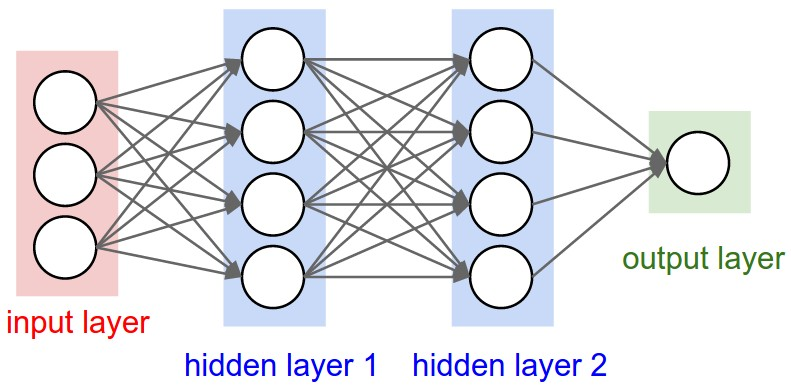
\includegraphics[width=0.75\linewidth]{Plantilla_TFG_latex//imagenes//Inf//2.Fund/neural_net2.jpeg}
    \caption[Estructura de una red neuronal profunda con dos capas ocultas]{Estructura de una red neuronal profunda con dos capas ocultas. La imagen representa una red neuronal artificial multicapa compuesta por una capa de entrada (\textit{input layer}, en rojo), dos capas ocultas (\textit{hidden layers}, en azul) y una capa de salida (\textit{output layer}, en verde). Cada neurona en una capa está completamente conectada con las neuronas de la siguiente capa mediante pesos sinápticos, representados por líneas. La capa de entrada recibe los datos del problema, las capas ocultas permiten la extracción de características y la modelización de relaciones complejas, y la capa de salida genera la predicción final. Esta arquitectura es típica en aprendizaje profundo y se entrena mediante algoritmos de optimización como el descenso de gradiente. Obtenida de \cite{stanford_231}.}
    \label{fig:NeuralNet}
\end{figure}


\subsection{Redes convolucionales}
\label{sec:convnets}

Las ConvNets o redes convolucionales son una familia de modelos de aprendizaje profundo usadas en la visión por computador. Obtienen un rendimiento al nivel del estado del arte en tareas como el reconocimiento de imágenes o la detección de objetos. Se caracterizan por tener una o varias capas (al menos una) basadas en convoluciones para luego tener una o varias capas totalmente conectadas. Las primeras sirven como extractores de características que capturan propiedades espaciales de las imágenes, mientras que las segundas sirven para clasificación \cite{GoodFellowBook}.

\subsubsection{Operación de convolución}

La convolución es una operación matemática que expresa la relación entre la entrada, la salida y la respuesta del sistema a los impulsos. En el contexto del procesamiento de señales, la convolución combina dos señales para producir una tercera \cite{GoodFellowBook}. Se define matemáticamente para funciones continuas como

$$ (f \ast g)(t) = \int_{-\infty}^{\infty} f(x)g(t-x)dx.$$

Para funciones discretas se define como

$$ (f \ast g)(t) = \sum_{x=-\infty}^{\infty} f(x)g(t-x).$$

Nos referimos a $f$ como la entrada y a $g$ como el núcleo o filtro. En el aprendizaje automático la entrada suele ser un tensor de datos y el filtro un tensor de parámetros que adaptamos con el algoritmo de aprendizaje. Ambos son de dimensión finita y asumimos que su valor es 0 en todos los puntos donde no almacenamos su valor. Por tanto en la práctica podemos implementar la sumatoria infinita como una suma finita de los elementos de un vector. Si usamos una imagen bidimensional $I$ como entrada, seguramente usaremos un filtro bidimensional $K$:

$$S(i,j) = (I \ast K)(i,j) = \sum_m \sum_n I(m,n)K(i-m,j-n).$$


Las convoluciones cumplen las siguientes propiedades:

\begin{itemize}

	\item \textbf{Conmutatividad}: $f \ast g = g \ast f$.
	
	\item \textbf{Asociatividad}: $f \ast (g \ast h ) = ( f \ast g) \ast h$.
	
	\item \textbf{Distributividad}: $f \ast (g + h) = (f \ast g) + (f \ast h)$.

\end{itemize}

La propiedad conmutativa es útil a nivel matemático pero no es demasiado práctica en la implementación de una red neuronal. Por ello muchas librerías de aprendizaje automático optan por implementar la función llamada relación cruzada en lugar de la convolución, volteando el núcleo como podemos ver en la Figura \ref{fig:3.Conv}.

$$C(i,j)= (I \cdot K)(i,j) = \sum_m \sum_n I(i+m,j+n)K(m,n).$$


\begin{figure}
    \centering
    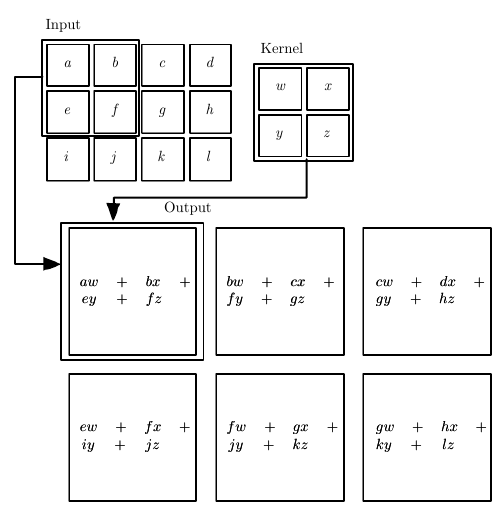
\includegraphics[width=0.5\linewidth]{Plantilla_TFG_latex//imagenes//Inf//2.Fund/Conv.png}
    \caption[Operación de correlación cruzada en una red neuronal convolucional]{Operación de correlación cruzada en una red neuronal convolucional. La imagen ilustra el proceso de correlación cruzada (\textit{cross-correlation}), una operación fundamental en redes neuronales convolucionales (ConvNets), y que es equivalente a la operación de convolución pero sin voltear el filtro. Se muestra una matriz de entrada (\textit{Input}) de 
$3 \times 4$ con elementos etiquetados ($a$ a $l$) y un kernel o filtro (\textit{Kernel}) de $2 \times 2$ con pesos ($w,x,y,z$). La operación consiste en deslizar el kernel sobre la matriz de entrada, calculando productos ponderados entre los valores superpuestos y sumando los resultados para formar la matriz de salida (\textit{Output}). Cada celda en la matriz de salida representa la suma de productos en una región local de la entrada. Este proceso permite la extracción de características espaciales en imágenes, siendo una base fundamental en la detección de patrones en ConvNets. Obtenida de \cite{GoodFellowBook}.}
    \label{fig:3.Conv}
\end{figure}


Al igual que hacen estas librerías, llamamos a estas dos operaciones indistintamente convolución, ya que en el contexto del aprendizaje de modelos no habrá diferencia, porque el algoritmo de aprendizaje obtendrá los mismos valores para el núcleo y sólo variará su posición. Podemos considerar la convolución como una multiplicación matricial donde la matriz tiene restricciones en muchas posiciones las cuales deben tener el mismo valor.

\subsubsection{Capa Convolucional}


Las capas convolucionales son las más importantes en la arquitectura de una ConvNet. Las claves de su gran rendimiento en el campo de la visión por computador son: la conectividad local, la disposición espacial y compartir parámetros \cite{GoodFellowBook}.

La conectividad local hace referencia a las conexiones de las neuronas. En entradas de alta dimensionalidad como imágenes no es práctico conectar una neurona con todas las neuronas del volumen anterior, por tanto cada neurona se conecta solo a una región local del volumen de entrada. Esto viene determinado por un hiperparámetro llamado campo receptivo, que es el tamaño del filtro que aplicamos. Mientras que las conexiones son locales en el espacio 2D (ancho y altura), siempre abarcan toda la profundidad del volumen de entrada.

Con la disposición espacial nos referimos al tamaño del volumen de salida y cómo están organizadas estas neuronas. Hay tres hiperparámetros con los que controlamos esto:

\begin{enumerate}

	\item Profundidad del volumen de salida: corresponde a la cantidad de filtros que queremos usar.
	
	\item \textit{Stride}: Indica el número de píxeles (hablando en términos de imágenes) que usamos para desplazar el filtro al realizar la convolución.
	
	\item \textit{Padding}: A veces, para mantener la dimensión de la salida es conveniente rellenar el borde de la entrada con ceros.

\end{enumerate}


Las dimensiones del volumen de salida podemos calcularlas como una función dependiente del tamaño del volumen de entrada $W$, el tamaño del filtro $F$, el \textit{stride} $S$ y el \textit{padding} $P$ que queramos aplicar. La fórmula es la siguiente:

\begin{equation}\label{eq:output}
\frac{W-F-2P}{S+1}.
\end{equation}

Esta nos dará las dimensiones en ancho y altura del volumen de salida como podemos ver en la Figura \ref{fig:stride}, y su profundidad vendrá totalmente determinada por el número de filtros que queramos usar.

\begin{figure}
    \centering
    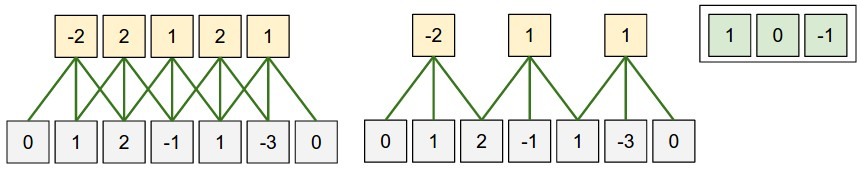
\includegraphics[width=0.75\linewidth]{Plantilla_TFG_latex//imagenes//Inf//2.Fund/2.stride.jpeg}
    \caption[Proceso de convolución en una red neuronal convolucional]{La imagen ilustra el proceso de convolución en una red neuronal convolucional. Los rectángulos grises representan las entradas, mientras que los vectores amarillos son las salidas resultantes de convolucionar las entradas con el filtro (ubicado en la esquina superior derecha). Los tamaños de las salidas pueden calcularse según la fórmula \ref{eq:output}. El filtro de tamaño $1 \times 3$ tiene valores [1, 0, -1]. El concepto de \textit{padding}, visible como bordes adicionales alrededor de las entradas, se utiliza para controlar el tamaño de las salidas. En ninguno de los dos ejemplos se usa ($P=1$). El \textit{stride}, o desplazamiento del filtro, determina cómo el filtro se mueve a través de las entradas, afectando el solapamiento y el tamaño resultante de las salidas. En el ejemplo de la izquierda se usa un \textit{stride} de $S=1$, mientras que en el de la derecha se usa $S=2$. Estos conceptos son esenciales en el aprendizaje profundo, ya que permiten ajustar la resolución y características extraídas por las ConvNets. Obtenida de \cite{stanford_231}.}
    \label{fig:stride}
\end{figure}


Compartir parámetros en una ConvNet nos permite reducir el número de éstos, reduciendo el coste del entrenamiento. Se basa en la suposición de que si una característica es útil en una posición espacial $(x,y)$ tambien lo será en otra cercana $(x',y')$. En un volumen $W \times H \times D$, en lugar de que cada neurona tenga su conjuntos de pesos, tenemos $D$ conjuntos de pesos, reduciendo drásticamente su número. 

\subsubsection{Capa \textit{Pooling}}

Su función es reducir progresivamente el tamaño de la representación para reducir el número de parámetros y la carga computacional en la red, además de controlar el sobreajuste. Opera independientemente a lo largo de la profundidad del volumen, usando la operación máximo. La opción más común es usar filtros $2 \times 2$ con un \textit{stride} $S= 2$ como se observa en la Figura \ref{fig:pooling}. La dimensión de la profundidad permanece intacta. Existen otros tipos de \textit{pooling}, por ejemplo realizar la media entre los elementos, pero esta opción fue dejando paso a la de seleccionar el máximo ya que obtiene mejores resultados en la práctica \cite{stanford_231}.

\begin{figure}
    \centering
    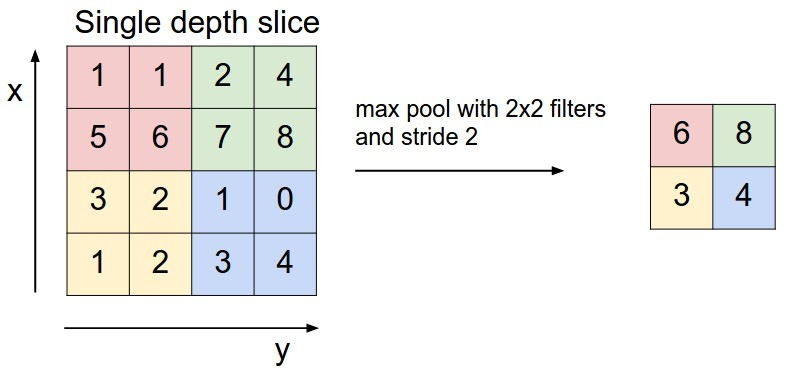
\includegraphics[width=0.75\linewidth]{Plantilla_TFG_latex//imagenes//Inf//2.Fund/maxpool.jpeg}
    \caption[Ejemplo de una operación \textit{max pooling} en una red convolucional]{La imagen muestra un ejemplo de una operación \textit{max pooling} en una ConvNet. A la izquierda, se presenta una matriz de 4x4 , con valores que van del 0 al 8. La operación de max pooling se realiza con filtros de $2\times 2$ y un \textit{stride} de 2, lo que significa que el filtro se mueve dos posiciones a la vez tanto en la dirección $x$ como en la dirección $y$. El resultado de esta operación se muestra a la derecha como una matriz de $2\times 2$, donde cada valor es el máximo de los valores en la correspondiente submatriz de $2\times 2$ de la original. Los valores resultantes son 6, 8, 3 y 4. Esta operación es relevante porque reduce la dimensionalidad de la entrada, manteniendo las características más importantes, lo que ayuda a disminuir el costo computacional y a evitar el sobreajuste en modelos de aprendizaje profundo. Obtenida de \cite{stanford_231}.}
    \label{fig:pooling}
\end{figure}

\subsubsection{Capa \textit{Batch Normalization}}

\textit{Batch Normalization} (BatchNorm) \cite{batchnorm} es un método de reparametrización adaptativa motivado por la dificultad de entrenar modelos muy profundos. En una capa de BatchNorm se estandariza la entrada a través de escalarla y trasladarla, lo que ayuda a estabilizar y acelerar el entrenamiento \cite{stanford_231}. Para cada \textit{mini-batch}, se realiza el siguiente proceso:

\begin{enumerate}

	\item Se calcula la media $\nu_{B}= \frac{1}{m} \sum_{i=1}^{m}x_i$ y la varianza $\sigma^{2}_B=\frac{1}{m} \sum_{i=1}^m(x_i - \nu_B)^2$.
	
	\item Se normaliza la entrada: $\hat{x}_i = \frac{x_i - \nu_B}{\sqrt{\sigma^{2}_B + \epsilon}}$, donde $\epsilon$ es una constante pequeña para evitar la división por 0.
	
	\item Se escala y se traslada la entrada normalizada: $y_i=\gamma \hat{x}_i + \beta$, donde $\gamma$ y $\beta$ son parámetros aprendibles por el modelo.
\end{enumerate}

Normalizando la entrada conseguimos hacer el proceso de entrenamiento más estable e intentar evitar el problema de la explosión o desvanecimiento del gradiente. También proporciona flexibilidad y mejora el rendimiento al reescalar y trasladar la entrada, y que esto dependa de parámetros aprendibles.

\subsubsection{Capa totalmente conectada}

Al final de las redes convolucionales lo más común es encontrarnos una o varias capas totalmente conectadas o \textit{fully connected} (FC), es decir, que cada neurona está conectada a todas las neuronas de la capa anterior, de la misma manera que ocurre en un MLP. Esta parte de la red permite clasificar las características extraídas por las capas convolucionales \cite{stanford_231}.

\subsection{\textit{Residual Networks}}
\label{sec:resnets}

Las \textit{Residual Networks} (ResNets) \cite{ResNets} son una familia de modelos dentro de las ConvNets que también usaremos en la experimentación, en versiones de 15 y 57 capas. Su característica principal es que usan bloques residuales, que agrupan varias capas en los cuales se suma la identidad (la entrada al bloque) a la salida del bloque. Que las redes neuronales profundas aprendan esta función identidad previene el problema de la degradación, es decir, que el rendimiento de la red decaiga a medida que aumenta el número de capas. Esto puede surgir por varias causas como la inicialización de los pesos, la función de activación o el desvanecimiento/explosión del gradiente \cite{divedeeplearning}. 

\subsubsection{Bloques residuales}

La función identidad se aprende a través de las conexiones residuales, que conectan el inicio y el final de los bloques residuales pasando la identidad. Estas conexiones además permiten aliviar el problema del desvanecimiento de gradiente. Vamos a centrarnos en una red neuronal de manera local, como se muestra en la Figura \ref{fig:resblock}. 

Si la función identidad $f(x)=x$ es el mapeo subyacente deseado, la función residual equivale a $g(x)=0$ y, por tanto, es más fácil de aprender: sólo tenemos que llevar a cero los pesos y sesgos de la última capa de pesos dentro de la línea de puntos. Con los bloques residuales, las entradas pueden propagarse más rápidamente a través de las conexiones residuales entre capas.

\begin{figure}
    \centering
    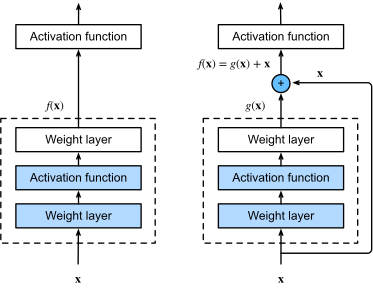
\includegraphics[width=0.75\linewidth]{Plantilla_TFG_latex//imagenes//Inf//2.Fund/resblock.png}
    \caption[Comparación entre una red neuronal tradicional y una red residual]{La imagen muestra una comparación entre una red neuronal tradicional y una red residual. En la red tradicional (izquierda), la entrada $x$ pasa a través de una capa de pesos y una función de activación para producir la salida $H(x)$. En la red residual (derecha), la entrada $x$ se suma a la salida de una capa de pesos y una función de activación, formando $H(x) + x$. Esta estructura de suma de atajos permite que la red residual aprenda funciones de identidad más fácilmente, lo que facilita el entrenamiento de redes profundas al mitigar el problema del desvanecimiento del gradiente. Obtenida de \cite{divedeeplearning}.}
    \label{fig:resblock}
\end{figure}

Para ello necesitamos que la entrada y la salida del bloque tengan el mismo tamaño. Si reducimos la dimensionalidad de la entrada o aumentamos el número de filtros entonces deberemos modificar la entrada a través de convoluciones $1 \times 1$ para que tenga el mismo tamaño que la salida, como se muestra en la Figura \ref{fig:resblock1x1}.

\begin{figure}
    \centering
    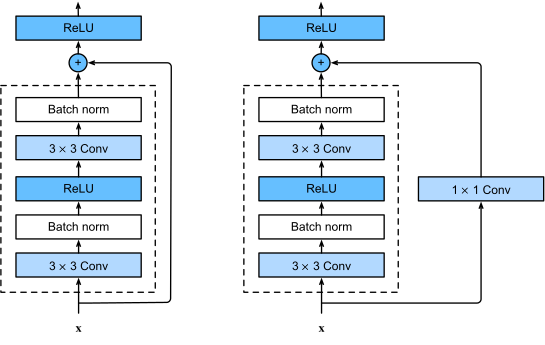
\includegraphics[width=0.75\linewidth]{Plantilla_TFG_latex//imagenes//Inf//2.Fund/resblock1x1.png}
    \caption[Bloques residuales utilizados en \textit{Residual Networks}]{La imagen muestra dos bloques residuales utilizados en ResNets. A la izquierda, se presenta un bloque residual básico que consiste en dos capas convolucionales de 3$\times$3 con una función de activación ReLU entre ellas, y una conexión de atajo que suma la entrada original al resultado de las convoluciones. A la derecha, se muestra un bloque residual con una convolución 1$\times$1 adicional, que se utiliza para ajustar las dimensiones de la entrada antes de la suma. Este bloque también incluye dos capas convolucionales de 3$\times$3 con funciones de activación ReLU entre ellas. La convolución 1x1 es crucial para permitir que la suma de la conexión de atajo sea posible cuando las dimensiones de la entrada y la salida no coinciden, mejorando así la capacidad de la red para aprender características complejas sin aumentar significativamente el costo computacional. Obtenida de \cite{divedeeplearning}.}
    \label{fig:resblock1x1}
\end{figure}

\subsubsection{Convoluciones 1x1}

%https://blog.paperspace.com/network-in-network-utility-of-1-x-1-convolution-layers/

Los bloques residuales nos permiten aumentar la profundidad de la red evitando ciertos problemas asociados, pero al añadir más capas estamos aumentando considerablemente el número de parámetros. Las convoluciones con tamaño de filtro $1 \times 1$ son una herramienta poderosa para reducir el número de parámetros manteniendo la expresividad de la red. Fueron presentadas en \cite{bottleorig}. Este tipo de convoluciones se realizan antes de realizar la convolución requerida, de manera que la dividamos en dos, una con tamaño de filtro 1 y la otra con el tamaño original.

\begin{ejemplo}
	Para ver la diferencia en el número de parámetros al usar esta herramienta, calcularemos los parámetros necesarios para realizar una convolución en el caso de tener $C=256$ canales de entrada, $O=512$ canales de salida y tamaño del filtro $F=3$.
	
	Si no usamos convoluciones $1 \times 1$, tendríamos $P= F \times F \times C \times O + O = 1.180.160$ parámetros.
	
	Usándolas debemos elegir un tamaño de filtro intermedio, por ejemplo $C'=64$. Aplicamos primero la convolución $1 \times 1$: $P'_1= 1 \times 1 \times C \times C' + C'=16.448$ parámetros. A continuación realizamos la convolución con el tamaño de filtro original: $P'_2: F \times F \times C' \times O + O=295.424$. En total, sumando las dos capas tendríamos $311.872$ parámetros, unas cuatro veces menos que en el caso anterior.
\end{ejemplo}



\subsection{Optimizadores basados en gradiente descendente}
\label{sec:gd}
Con el objetivo de intentar abordar los principales problemas del algoritmo de aprendizaje del GD se han propuesto en la literatura diversas variantes, modificando la regla de actualización de los pesos. Existen optimizadores de primer y segundo orden, en función de si hacen uso sólo de la información del gradiente o también de la matriz Hessiana, respectivamente. Vamos a ver en esta sección únicamente los de primer orden, y veremos un método de segundo orden en la sección siguiente como parte de una MH memética. Se dan tres enfoques en este ámbito: el uso de momento, tasas de aprendizaje adaptativas y la combinación de los dos anteriores. De cada uno hacemos hincapié en el que vamos a usar en el presente TFG, en orden respectivo: NAG, RMSProp, Adam y AdamW.

\subsubsection{NAG}

El algoritmo del GD es problemático en regiones de la función de error donde una dimensión tiene mucha más pendiente que otra, que son comunes alrededor de óptimos locales. En estos escenarios el algoritmo oscila y realiza poco progreso real. El momento \cite{momentumorig} es un método que acelera al algoritmo en la dirección relevante y compensa las oscilaciones, como podemos ver en la Figura \ref{fig:momentum}. Esto se realiza añadiendo una fracción $\gamma$ del vector gradiente de la última iteración al vector gradiente actual \cite{divedeeplearning, GoodFellowBook}.

\begin{figure}[!tbp]

  \centering
  \subfloat{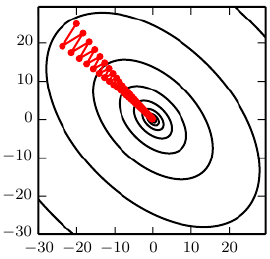
\includegraphics[width=0.4\textwidth]{Plantilla_TFG_latex//imagenes//Inf//2.Fund/sgdwoutmom.png}}
  \hfill
  \subfloat{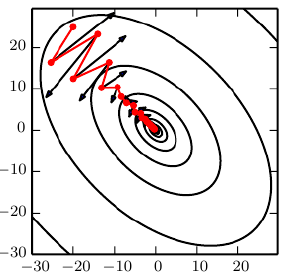
\includegraphics[width=0.4\textwidth]{Plantilla_TFG_latex//imagenes//Inf//2.Fund/sgdwmom.png}}
  \caption[Comparación entre el algoritmo de gradiente descendente estocástico original y usando el momento]{Comparación entre el algoritmo de GD estocástico original (izquierda) y usando el momento (derecha). Vemos que en la figura de la derecha se diferencia la dirección del gradiente (flechas negras) y el camino seguido por el algoritmo en rojo. Se observa que usando el momento se producen oscilaciones al principio que se van reduciendo a lo largo de la ejecución del algoritmo. Usando el momento se necesitan menos iteraciones para converger. Imágenes obtenidas de \cite{GoodFellowBook}.}
    \label{fig:momentum}
\end{figure}

\begin{align*}	
	v_t&= \gamma v_{t-1} + \eta \nabla C(W_t) \\
	W_{t+1} &= W_t- v_t. \\
\end{align*}

El valor de $\gamma$ se sitúa normalmente alrededor de 0.9. El término del momento se incrementa en las dimensiones en las que el gradiente apunta en la misma dirección y se reduce en las que el gradiente cambia de dirección, consiguiendo una convergencia más rápida y estable. Dotamos al algoritmo de cierta inercia para reducir la brusquedad en los cambios de dirección.

El optimizador \textit{Nesterov Accelerated Gradient} (NAG) \cite{Nesterov} modifica esta idea de manera que podamos ``predecir'' a dónde nos lleva esa inercia. A la hora de calcular el gradiente de la función de coste, no lo hacemos respecto a los parámetros, sino respecto a una aproximación de los parámetros tras la iteración actual, de manera que podamos saber de forma aproximada dónde nos encontraremos después de actualizar los pesos. Se puede interpretar como una corrección del método de momento original. El valor del momento se sitúa también alrededor de 0.9.

\begin{align*}	
	v_t&= \gamma v_{t-1} + \eta \nabla C(W-v_t) \\
	W_{t+1} &= W_t - v_t. \\
\end{align*}

Mientras que usando el optimizador momento original primero calculamos el gradiente y luego realizamos un salto grande en la dirección del gradiente acumulado, NAG primero realiza un salto grande en la dirección del gradiente acumulado, mide el gradiente y despúes realiza una corrección. Esta comparación se ilustra en la Figura \ref{fig:NAG}. Esta estrategia previene al algoritmo de avanzar demasiado rápido. 

\begin{figure}
    \centering
    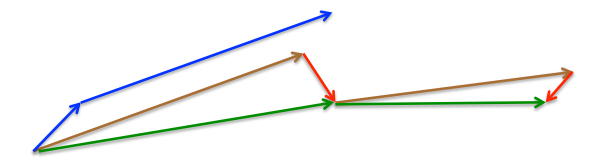
\includegraphics[width=0.75\linewidth]{Plantilla_TFG_latex//imagenes//Inf//2.Fund/NAG.png}
    \caption[Comparación del cálculo del tamaño del paso entre los métodos del momento original y el momento de Nesterov]{Comparación entre los métodos del momento original (vectores azules) y el momento de Nesterov, que muestra el paso en dos iteraciones del algoritmo de GD para mostrar las diferencias en su cálculo. En este último, primero realizamos un salto grande en la dirección del gradiente acumulado (vector marrrón) para luego medir el gradiente de la posición al acabar el salto y realizar una corrección (vector rojo). La flecha verde indica la posición final corregida donde acaba una iteración del método NAG. Obtenida de \cite{rmsprop}.}
    \label{fig:NAG}
\end{figure}


\subsubsection{RMSProp}

RMSProp (Root Mean Square Propagation) es un optimizador de primer orden que introduce tasas de aprendizaje adaptativas. Presentado por Geoff Hinton en sus materiales docentes \cite{rmsprop}, la fórmula de actualización de los pesos es la siguiente:

\begin{align*}
	E[g]_t &= 0.9 E[g]_{t-1} + 0.1 \nabla C(W_t)^{2}\\
	W_{t+1} &= W-t - \frac{\eta}{\sqrt{E[g_t^2]_t + \epsilon}}\nabla C(W_t)
\end{align*}

Donde $E[g^2]_t$ es la media móvil en la iteración $t$, que depende solamente de la iteración anterior y del gradiente actual. Las operaciones anteriores se realizan elemento a elemento, es decir, cada peso recibe una actualización con un factor personalizado. Actualizando los pesos de esta forma, cuando el gradiente es grande en una dirección entonces el factor de ese peso será pequeño, evitando oscilaciones; mientras que si en otra dirección el gradiente es relativamente pequeño entonces el valor será grande, acelerando el proceso de entrenamiento.

Existen otros optimizadores que usan tasas de aprendizaje variables como Adagrad \cite{adagrad}, sus diferencias residen en la ventana de iteraciones y el cálculo del factor de multiplicación del peso. En este optimizador sólo se tienen en cuenta la iteración pasada y la actual, mientras que el uso de una media exponencial decreciente permite que las tasas de aprendizaje no se vuelvan demasiado pequeñas \cite{divedeeplearning, GoodFellowBook}.

\subsubsection{Adam}

\textit{Adaptative Moment Estimation} (Adam) \cite{Adam} es otro método que calcula tasas de aprendizaje adaptativas para cada parámetro. Además mantiene una media exponencial decreciente de gradientes de iteraciones anteriores $m_t$ similar al momento.

\begin{align*}
	m_t&= \beta_1 m_{t-1} + (1-\beta_1)\nabla C(W) \\
	v_t&= \beta_2 v_{t-1} + (1-\beta_2)\nabla C(W)^2.
\end{align*}

$m_t$ y $v_t$ son estimaciones del momento de primer orden (media) y de segundo orden (varianza no centrada) de los gradientes, respectivamente. Son inicializados como vectores de 0, por lo que sus autores encontraron que tenían un sesgo al 0, especialmente durante las primeras iteraciones y cuando $\beta_1$ y $\beta_2$ son próximos a 1. Por tanto se calculan nuevas variables corrigiendo el sesgo:

\begin{align*}
	\hat{m}_t&=\frac{m_t}{a-\beta_1}\\
	\hat{v}_t&=\frac{v_t}{1-\beta_2}.
\end{align*}

Ahora se usan para ajustar los parámetros como hemos visto en el optimizador anterior:

$$W_{t+1} = W_t - \frac{\eta}{\sqrt{\hat{v}_t} + \epsilon} \hat{m}_t$$

Los autores proponen valores por defecto de 0.9 para $\beta_1$, 0.999 para $\beta_2$ y $10^{-8}$ para $\epsilon$ \cite{divedeeplearning, GoodFellowBook}.

\subsubsection{AdamW}

AdamW (Adam con Weight decay) \cite{AdamW} es una modificación de Adam que arregla un error de implementación, desacoplando la regularización de la actualización del gradiente. En lugar de incorporar el decaimiento de pesos en el cálculo de gradiente, como en Adam original, AdamW directamente modifica los parámetros tras el paso de actualización del gradiente añadiendo una pequeña fracción del término de decaimiento de pesos, lo que conlleva una regularización más efectiva.


$$W_t = W_{t-1} - \eta \cdot \frac{\hat{m}_t}{\sqrt{\hat{v}_t} + \epsilon} - \lambda \cdot W_{t-1}$$

\subsubsection{L-BFGS-B}\label{sec:l-bfgs}


En el presente TFG utilizamos L-BFGS-B no como optimizador a utilizar en la experimentación, sino como componente del algoritmo SHADE-ILS. Aun así, este es en sí mismo un optimizador basado en gradiente, por lo cual aparece en esta sección.

El método L-BFGS-B (\textit{Limited-memory Broyden-Fletcher-Goldfarb-Shanno with Box constraints}) \cite{L-BFGS-B} es un algoritmo Quasi-Newton, es decir, un algoritmo de optimización iterativo. Los métodos de Newton usan la matriz Hessiana de la función a optimizar para usar más información del problema y ofrecer una convergencia más rápida y estable. Para problemas complejos de  dimensionalidad elevada, calcular la Hessiana en cada paso es una tarea computacionalmente inabarcable, y los métodos de Quasi-Newton implementan una aproximación de la Hessiana para rebajar esta carga computacional. Estos métodos se diferencian entre ellos principalmente en la forma de aproximar la matriz Hessiana \cite{Numerical_optimization}.

Uno de los métodos Quasi-Newton más populares es BFGS \cite{BFGS}, que usa una aproximación de la Hessiana de forma que mantiene su propiedad de definida positiva, lo que asegura una convergencia estable. Sin embargo, aunque se reduce el coste computacional, para almacenar la matriz Hessiana se requiere demasiada memoria. El método L-BFGS \cite{L-BFGS}, en lugar de guardar una matriz con $n \times n$ aproximaciones, guarda únicamente un vector de tamaño $n$ que guarda todas las aproximaciones de manera implícita. Esta variante está diseñada para problemas de alta dimensionalidad, y produce resultados similares a su versión sin la memoria limitada \cite{stanford_231}.

La última variante L-BFGS-B, que usamos en el presente TFG en el algoritmo SHADE-ILS, es una modificación que maneja restricciones en los valores de las variables, lo que la hace incorporar información sobre el dominio. Al usar información del gradiente y de la Hessiana, es un optimizador de segundo orden, aunque es mucho menos popular que los optimizadores de primer orden. Aunque mejora la rapidez y estabilidad de la convergencia al usar más información del problema y proporciona mejores soluciones, los problemas de aprendizaje automático a día de hoy han adquirido una dimensionalidad demasiado alta para que este tipo de métodos resulten computacionalmente asequibles, y se prefiere usar los de primer orden. Aún así vemos que se implementa dentro del algoritmo de SHADE-ILS con resultados muy satisfactorios, no usándose como método de optimización principal sino de manera complementaria al algoritmo SHADE \cite{Numerical_optimization}.


\subsection{Metaheurísticas}
\label{sec:mh}

En su definición original las MH son métodos que combinan técnicas de mejora local con estrategias de alto nivel para crear un proceso capaz de escapar óptimos locales y realizar una búsqueda robusta del espacio de soluciones. Aunque no hay garantía teórica de que puedan encontrar la solución óptima, su rendimiento es muy superior en algunos casos al de algoritmos exactos que requieren demasiado tiempo para completar su ejecución, especialmente en problemas complejos del mundo real. En problemas NP-Difícil por ejemplo se prioriza el uso de MH que dan una solución cercana a la óptima en un tiempo mucho menor que algoritmos exactos \cite{mhhandbook}.

Podemos clasificar a las MH en dos grandes grupos en función de cómo se realiza la búsqueda por el espacio de soluciones: basadas en trayectorias y basadas en poblaciones. En las primeras el proceso de búsqueda se caracteriza por realizar una trayectoria en el espacio de búsqueda, que puede ser visto como la evolución en tiempo discreto de un sistema dinámico. En las MH basadas en poblaciones, en cada iteración hay un conjunto de soluciones que interactúan entre sí. Nos centraremos en este último tipo ya que es el que vamos a usar \cite{mhhandbook}.

\subsubsection{Metaheurísticas basadas en poblaciones}

Son técnicas de optimización probabilística que con frecuencia mejoran a otros métodos clásicos, e intentan imitar el mecanismo de evolución de la naturaleza a través de similitudes con la genética, como se ilustra en la Figura \ref{fig:cruce_mh}. Tiene un conjunto de soluciones denominado población, donde cada solución se llama individuo, y son generados de forma aleatoria. En cada iteración o generación, estos individuos se recombinan entre sí para intentar obtener mejores soluciones cuyo rendimiento es medido con una función objetivo. Las etapas de cada generación se pueden ver esquemáticamente en la figura \ref{fig:gen_alg}, y son:

\begin{figure}
    \centering
    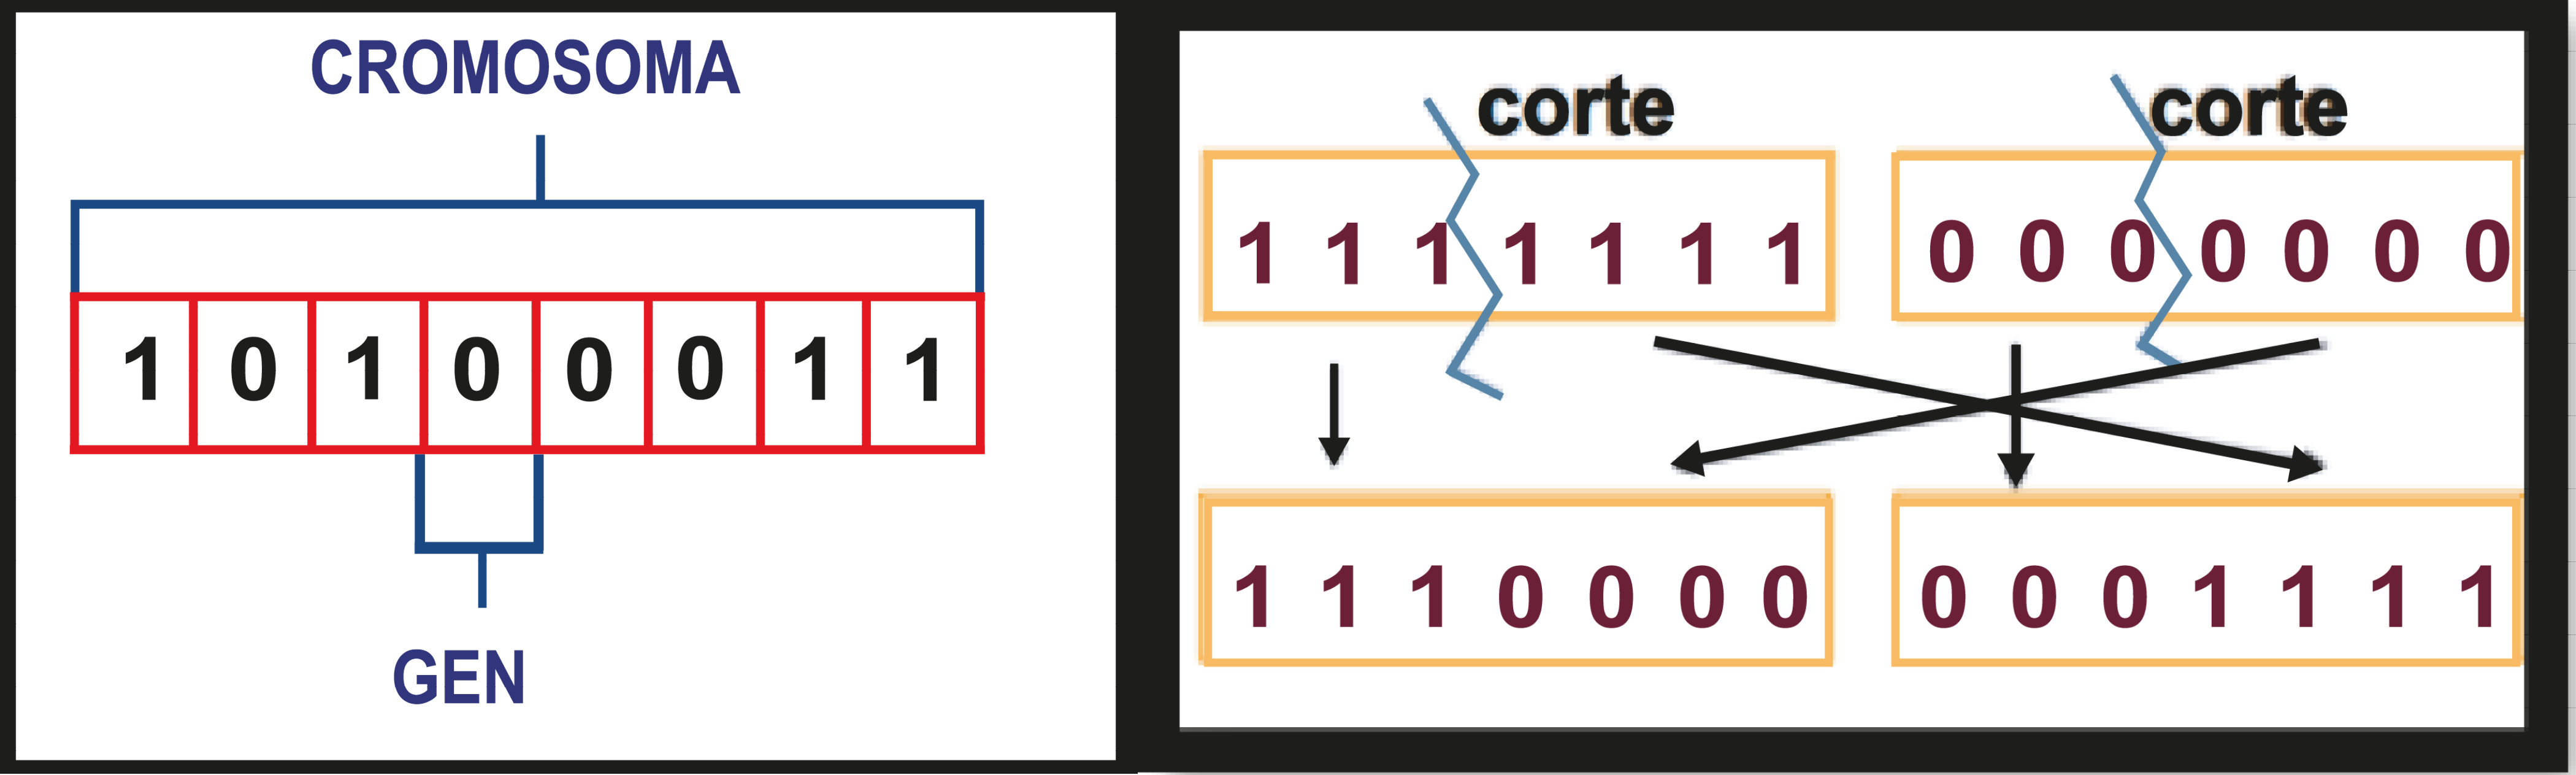
\includegraphics[width=0.75\linewidth]{Plantilla_TFG_latex//imagenes//Inf//2.Fund/cruce_mh.png}
    \caption[Representación y cruce de cromosomas en algoritmos genéticos]{La imagen ilustra la representación y el proceso de cruce de cromosomas en algoritmos genéticos. A la izquierda, se muestra un cromosoma compuesto por una cadena de bits (1 y 0) en la parte superior destacando un gen específico dentro del cromosoma. A la derecha, se presenta el proceso de cruce (corte) entre dos cromosomas parentales a través del operador de cruce en un punto. Los cromosomas parentales, representados por las cadenas '1111111' y '0000000', se cortan en un punto específico, intercambiando segmentos para formar dos nuevos cromosomas hijos: '1110000' y '0001111'. Este proceso es fundamental en los algoritmos genéticos, ya que permite la combinación y variación de información genética para la optimización y solución de problemas complejos.}%https://revistamarina.cl/es/articulo/metodos-metaheuristicos-caso-algoritmos-geneticos-en-construccion-naval
    \label{fig:cruce_mh}
\end{figure}

\begin{itemize}
	\item Selección: se elige una parte de la población actual, normalmente con criterios elitistas (se elige a los mejores) aunque introduciendo cierta aleatoriedad. Si el número de individuos elegidos es igual al tamaño de la población, hablamos de un modelo generacional, mientras que si es menor hablamos de un modelo estacionario. 
	\item Cruce: Los individuos seleccionados se agrupan por parejas y se combinan a través del operador de cruce. Las soluciones resultantes se denominan hijos. Operadores comunes son el cruce en un punto, el cruce en dos puntos y el cruce uniforme. 
	\item Mutación: A los hijos se les aplican cambios aleatorios en sus valores para mantener cierta diversidad genética en la población.
	\item Reemplazo: Se reemplaza la población actual con la nueva generación. Podemos reemplazarla entera o aplicar criterios elitistas, como reemplazar sólo con los mejores o reemplazar sólo si la nueva generación es mejor que la anterior.
	\item Terminación: se comprueba si se cumple la condición de parada. Criterios comunes son un número máximo de iteraciones o la convergencia de la población (falta de mejoras entre generaciones).
\end{itemize}

\begin{figure}
    \centering
    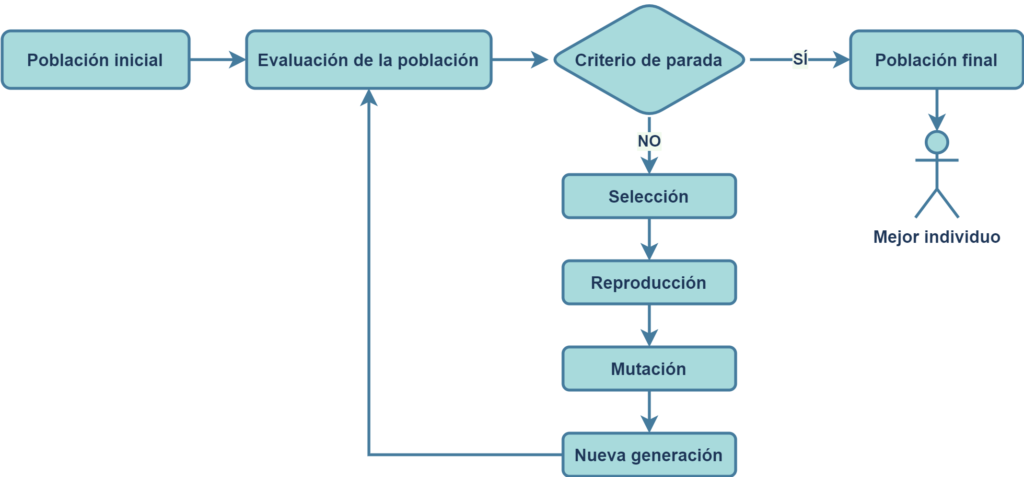
\includegraphics[width=0.75\linewidth]{Plantilla_TFG_latex//imagenes//Inf//2.Fund/alg_gen.png}
    \caption[Etapas de un algoritmo genético]{La imagen presenta un diagrama de flujo de un algoritmo genético, que incluye los siguientes pasos: iniciar con una ``Población inicial'', donde se crea una población de posibles soluciones, que se somete a una ``Evaluación de la población'', en la que cada individuo se puntúa según una función objetivo. Si se cumple el ``Criterio de parada'', se obtiene la ``Población final'' y se identifica el ``Mejor individuo''. Si el criterio no se cumple, se procede a la ``Selección'' de individuos, donde se seleccionan los individuos que se reproducirán a través de un proceso predefinido que asegure diviersidad en la población y buenas solucions, seguida de los procesos de ``Reproducción'' y ``Mutación'', en los que se cruzan los individuos seleccionados y luego se les aplica una pequeña modificación, respectivamente; para generar una ``Nueva generación''. Este ciclo se repite hasta que se cumple el criterio de parada, optimizando las soluciones tras cada generación. Obtenida de \url{https://blogs.imf-formacion.com/blog/tecnologia/}}
    \label{fig:gen_alg}
\end{figure}

Los criterios elitistas hacen que la convergencia sea más rápida, pero podemos caer en una convergencia prematura por la falta de diversidad que conllevan estos criterios, de manera que nuestro algoritmo pare antes de encontrar una solución lo suficientemente buena.



\subsubsection{\textit{Differential Evolution}}


Los algoritmos de DE \cite{diffev} son modelos basados en poblaciones que son particularmente efectivos para problemas de optimización continuos. Enfatizan la mutación y la realizan antes de aplicar el operador de cruce. Usan los parámetros factor de mutación $F$ y probabilidad de cruce $C_r$ \cite{diffevbook}. Las etapas que varían, descritas en el orden que se realizan en cada generación, son las siguientes:

\begin{itemize}
	\item{Operador de mutación: Para cada solución $x_i$ de la población, se genera un vector mutante $v_i$ a partir de la siguiente expresión:
	
	$$v_i = x_{r1} + F \cdot (x_{r2} - x_{r3}).$$
	
	Donde $x_{r1}, x_{r2}$ y $x_{r3}$ son individuos seleccionados aleatoriamente con las restricciones de que $x_i  \neq x_{rj}$ y $x_{rj} \neq x_{rj'}$ con $j, j' \in \left \{ 1,2,3 \right \}$. $F$ se suele situar en la práctica ente 0 y 2.		
	}
	
	\item{Cruce: se combinan el vector solución de partida $x_i$ y el vector mutante $v_i$ para generar el vector de prueba $u_i$. Se usa el cruce binomial:
	
	$$u_{ij} = \begin{cases}
		v_{ij} & \text{si } \text{rand}_j(0,1) \leq C_r \\
		x_{ij} & \text{en otro caso}
		\end{cases} $$
		
		donde $\text{rand}_j(0,1)$ es generado aleatoriamente con una distribución uniforme entre 0 y 1 para cada componente $j$.	
	}
	
	\item{Selección: se compara el valor de la función objetivo de los vectores iniciales con el de los vectores de prueba correspondientes, y el que tenga mayor valor pasa a la generación siguiente.}

\end{itemize}

En el pseudocódigo del Algoritmo \ref{alg:de} podemos apreciar el cambio de orden en las etapas de cada generación con respecto al esquema general de los algoritmos basados en poblaciones que veíamos en la Figura \ref{fig:gen_alg}.

\begin{algorithm}
\caption{Esquema general de DE}
\label{alg:de}
	\begin{algorithmic}
		\State $t:=0$
		\State Inicializar Pob$_t$
		\State Evaluar $x \quad \forall x \in$ Pob$_t$
		\While{No se cumpla condición de parada}
			\State $t:=t+1$			
			\State Mutar Pob$_t$ para obtener Pob'
			\State Recombinar Pob' y Pob para obtener Pob'' 
			\State Evaluar Pob''			
			\State Reemplazar Pob$_t$ a partir de Pob'' y Pob$_{t-1}$
		\EndWhile
		
		
		\Return $x_i \in Pob_t : f(x_i)\leq f(x_j)$
	\end{algorithmic}
\end{algorithm}		
		
	



\subsubsection{SHADE}

SHADE (\textit{Success-History based Adaptative Differential Evolution}) \cite{shade} es una variante avanzada del algoritmo original de DE. Consigue mejorar éste a través de guardar información histórica sobre configuraciones de los parámetros de factor de mutación ($F$) y el ratio de cruce ($CR$) que han tenido buenos resultados para poder ajustar de manera adaptativa estos parámetros y guiar el proceso de evolución, su pseudocódigo puede observarse en el Algoritmo \ref{alg:shade}. 

Los mecanismos de cruce y de selección son los mismos que en DE, variando principalmente el mecanismo de mutación. Para generar el vector mutante $v_i$ a partir de la solución $x_i$, SHADE usa la siguiente estrategia\footnote{Esta es la estrategia original, existen más modificaciones, aunque basadas en esta propuesta}:

$$v_i = x_{r1} + F \cdot (x_p - x_i)  + F \cdot (x_{r1} - x_{r2}).$$

Donde $x_p$ es un individuo seleccionado aleatoriamente de entre los $p$ mejores de la población y que es distinto a $x_i$. También se verifica que $x_i  \neq x_{rj}$ y $x_{rj} \neq x_{rj'}$ con $j, j' \in \left \{ 1,2 \right \}$. En el algoritmo de SHADE se usa $p=1$, es decir, se elige al mejor individuo de la población.

El algoritmo inicia los parámetros de factor de mutación y ratio de cruce al valor 0.5, y los va adaptando según se va ejecutando. Para ello mantiene un archivo de memoria, que se actualiza al final de cada generación y en el que se guardan parejas de los valores de los dos parámetros que han dado lugar a mejores soluciones. Al actualizar el archivo se usa la media de Lehmer\footnote{$Lehmer(X) = \frac{\sum_{x\in X} x^2}{\sum_{x\in X} x}$}  de manera que se le da más peso a las parejas de parámetros que mejor rendimiento obtienen. Al comienzo de cada generación el algoritmo obtiene valores de $F$ y $C_r$ para cada individuo basándose en el archivo de memoria e introduciendo pequeñas modificaciones.


%REVISAR PSEUDOCODIGO
\begin{algorithm}
\caption{Algoritmo SHADE}
\label{alg:shade}
	\begin{algorithmic}
		\State $t:=0$
		\State Inicializar Pob$_t$
		\State Inicializar $A$ (archivo externo)
		\State Inicializar $M$ (memoria de parámetros)
		\State Evaluar $x \quad \forall x \in$ Pob$_t$
		\While{evals $<$ total\_evals}
			\State $t:=t+1$
			\State Seleccionar $p$ soluciones para la mutación
			\State Mutar Pob$_{t-1}$ para obtener Pob'
			\State Recombinar Pob' y Pob$_{t-1}$ para obtener Pob''
			\State Evaluar Pob''
			\State Actualizar $A$ y $M$ a partir de Pob'' y Pob$_{t-1}$
			\State Obtener Pob$_t$ a partir de Pob'' y Pob$_{t-1}$
		\EndWhile
		
		
		\Return $x_i \in$ Pob$_t : f(x_i) \leq f(x_j) \quad \forall j$
	\end{algorithmic}
\end{algorithm}

SHADE está basado en DE, una familia de algoritmos de optimización que ofrece muy buenos resultados con parámetros continuos. En este ámbito, SHADE obtiene resultados del estado del arte en espacios de búsqueda de media-alta dimensionalidad, aunque no tan alta como el caso del entrenamiento de modelos de aprendizaje profundo \cite{shade}. En tareas donde la dimensionalidad es muy eleveda como la optimización de parámetros de grandes modelos, su versión memética SHADE-ILS, que veremos a continuación, consigue muy buenos resultados.



\subsubsection{Algoritmos meméticos}

Los algoritmos meméticos son técnicas de optimización MH basadas en el interacción entre componentes de búsqueda globales y locales, y tienen la explotación de conocimiento específico del problema como uno de sus principios. De manera general se componen principalmente de un algoritmo basado en poblaciones al cual se le ha integrado un componente de búsqueda local \cite{mhhandbook}.

Su principal diferencia con los algoritmos evolutivos tradicionales es que usan de manera concienzuda todo conocimiento disponible acerca del problema. Esto no es algo opcional sino que es una característica fundamental de los algoritmos meméticos. Al igual que los algoritmos genéticos se inspiran en los genes y la evolución, estas estrategias se inspiran en el concepto de ``meme'', análogo al de gen pero en el contexto de la evolución cultural. Normalmente se llama ``hibridar'' a incorporar información del problema a un algoritmo de búsqueda ya existente y que no usaba esta información.

Esta característica de incorporar información del problema está respaldada por fuertes resultados teóricos. En el teorema \textit{No Free Lunch} \cite{nofreelunch} se establece que un algoritmo de búsqueda tiene un rendimiento acorde con la cantidad y calidad de información del problema que usa. Más precisamente, el teorema establece que el rendimiento de cualquier algoritmo de búsqueda es indistinguible de media de cualquier otro cuando consideramos el conjunto de todos los problemas. 

\subsubsection{SHADE-ILS}
\label{sec:shade-ils}


SHADE-ILS \cite{shadeils} es un algoritmo memético para problemas de optimización continua a gran escala. Combina la exploración del algoritmo basado en poblaciones SHADE, usado en cada generación para evolucionar a la población de soluciones, con la explotación de una búsqueda local que se aplica a la mejor solución que se tenga en esa generación. 

En la parte de búsqueda local, en el algoritmo original existe un mecanismo de elección para usar entre varias búsquedas locales, una de ellas L-BFGS-B. En el presente TFG se ha decidido usar sólo esta última, por facilidad de implementación y porque usa más información específica del problema. Por tanto no se detallará este mecanismo de elección entre búsquedas.

Las características fundamentales de esta técnica y que la diferencia con respecto a otros algoritmos meméticos son la elección de los algoritmos empleados (tanto el de búsqueda local como el basado en poblaciones) y su mecanismo de reinicio. Éste se activa cuando a lo largo de tres generaciones el rendimiento de la mejor solución no supera en más de un 5\% al de la anterior. En dicho caso, se elige una solución aleatoria de la población y se le aplica una pequeña perturbación usando una distribución normal y el resto de la población se vuelve a generar aleatoriamente. Cuando ocurre esto los parámetros adaptativos son reiniciados a los valores por defecto.

Cabe destacar que esto se realiza ya que SHADE-ILS mantiene los parámetros adaptativos del algoritmo SHADE entre generaciones. Esto tiene mucho sentido ya que al finalizar una ejecución de dicho algoritmo, sólo aplicamos búsqueda local a una solución, con lo que la gran mayoría de la población queda intacta y por tanto podemos reutilizar estos parámetros que se han ido adaptando a ella. 

SHADE-ILS mantiene un variable para guardar la mejor solución hasta ahora y otra para guardar la mejor solución desde el último reinicio, devolviendo la primera cuando finaliza el algoritmo. En la versión utilizada se ha añadido además un array para guardar el histórico de las mejores soluciones junto con su fitness correspondiente, de manera que podamos analizar y representar las mejoras que realiza el algoritmo. 


\begin{algorithm}
\caption{Algoritmo SHADE-ILS}
\label{alg:shade-ils}
	\begin{algorithmic}
		\State $t := 0$
		\State Inicializar Pob$_t$
		\State $x_0 :=$ (maximo+minimo)/2
		\State $x_{\text{best}} := \text{L-BFGS-B}(x_0)$
		\State $x_{\text{global}} := x_{\text{best}}$
		
		\While{evals $<$ total\_evals}
			\State $t := t+1$
			\State $f_{\text{prev}} := f(x_{\text{best}})$
			\State $x_{\text{best}}, \text{Pob}_t := \text{SHADE}(\text{Pob}_{t-1})$
			\State $x_{\text{best}} := \text{L-BFGS-B}(x_{\text{best}})$
			\State $\Delta f := \frac{f_{\text{prev}} - f(x_{\text{best}})}{f_{\text{prev}}} \times 100$
			
			\If{$f(x_{\text{best}}) < f(x_{\text{global}})$}
				\State $x_{\text{global}} := x_{\text{best}}$
			\EndIf
			
			\If{$\Delta f < 5$}
				\State $g := g + 1$
			\Else
				\State $g := 0$
			\EndIf
			
			\If{$g \geq 3$}
				\State Reiniciar población conservando $x_{\text{best}}$ con perturbación normal
				\State $g := 0$
			\EndIf	
		\EndWhile
		
		\Return $x_{\text{global}}$
	\end{algorithmic}
\end{algorithm}


Vemos el pseudocódigo de la implementación realizada en el Algoritmo \ref{alg:shade-ils} y aclaramos algunas cosas que pueden no haber quedado del todo claras en favor de la claridad del pseudocódigo. Cuando generamos la población inicial, seleccionamos la peor y la mejor solución y la combinamos haciendo una media de sus elementos. A esa solución se le aplica la búsqueda local y se incluye en la población reemplazando a la peor solución. Se guardan los valores de mejora de las últimas 3 generaciones y en caso de que todas estén por debajo del 5\% se activa el mecanismo de reinicio.



En el artículo su publicación \cite{shadeils} se atienden tres cuestiones, todas a través de técnicas MH: diseño de la arquitectura, optimización de hiperparámetros y entrenamiento de los parámetros de un modelo. Nos centraremos en la última. Se utilizan seis conjuntos de datos distintos con diferente complejidad, y en base a ésta, se elige una arquitectura de modelo concreta dentro de la familia de las ConvNets, de manera que tenga buen rendimiento en su entrenamiento a través de GD. Se utiliza el optimizador Adam. En el entrenamiento con SHADE-ILS se utilizan diferentes estrategias que hacen uso de la estructura por capas de los modelos de aprendizaje profundo, realizando el entrenamiento en los pesos de diversas capas, según la estrategia, mientras se mantienen congelados los demás. También se realiza el entrenamiento de todo el modelo a la vez.

Los resultados de la experimentación son claros: solo en una de las seis tareas el modelo entrenado con SHADE-ILS minimiza más la función de pérdida que el modelo entrenado con GD. Además, en todos los casos, el error de test es mayor. Cabe mencionar que la generalización en los modelos es bastante buena, manteniéndose estos errores en valores cercanos a los que se obtiene en el entrenamiento, y aumentando el error en proporciones similares a lo que lo hace el modelo entrenado con Adam.

\subsection{Tests estadísticos}

Un test estadístico es una herramienta utilizada para evaluar hipótesis sobre una población basada en una muestra de datos. Formalmente, un test estadístico se define como un procedimiento que, dado un conjunto de datos observados, proporciona una regla de decisión para aceptar o rechazar una hipótesis nula $H_0$, en función de la evidencia contenida en los datos. La hipótesis alternativa $H_1$ representa la afirmación contraria a $H_0$.

El p-valor representa la probabilidad de obtener un resultado tan extremo como el observado, bajo la suposición de que la hipótesis nula es verdadera. En otras palabras, mide la evidencia en contra de $H_0$: valores pequeños de $p$ indican que la muestra es poco probable, lo que respalda la hipótesis alternativa $H_1$. Generalmente, se establece un umbral de significancia $\alpha$, comúnmente 0.05 o 0.01, y para p-valores por debajo de ese umbral se rechaza la hipótesis nula.

Los tests estadísticos pueden clasificarse en diferentes categorías según su propósito, como tests paramétricos y no paramétricos, tests de comparación de medias, tests de independencia y tests de ajuste a una distribución específica. Los tests paramétricos asumen que los datos provienen de una distribución específica con ciertos parámetros desconocidos, los cuales se estiman a partir de la muestra. Estos tests suelen ser más potentes cuando se cumplen sus supuestos, como la normalidad de los datos.

\subsubsection{Test de Shapiro-Wilk}

Sea $X= \left \{x_1, x_2,,\ldots,x_n \right \}$ una muestra de tamaño $n$ proveniente de una distribución desconocida. El test paramétrico de Shapiro-Wilk \cite{S-Wtest} evalúa la hipótesis nula $H_0$ de que la muestra sigue una distribución normal:

$$H_0: X \sim \mathcal{N}(\mu,\sigma^2), \qquad H_1: X \nsim \mathcal{N}(\mu,\sigma^2).$$

El estadístico $W$ se define como $W=\frac{\left( \sum_{n}^{i=1}a_ix_i \right) ^2}{\sum_{n}^{i=1} \left( x_i - \bar{x}  \right) ^2}$ donde:

\begin{itemize}

\item $x_i$ son los valores de la muestra ordenados de manera creciente.

\item $\bar{x}$ es la media muestral.

\item $a_i$ son coeficientes óptimos predefinidos que dependen de la media, varianza y covarianza de los orden estadísticos de una muestra de tamaño  proveniente de una distribución normal .

\end{itemize}


\subsubsection{Test de los rangos con signo de Wilcoxon}\label{sec:tests}

El test de los rangos con signo de Wilcoxon \cite{Wilcoxon} es una prueba estadística no paramétrica que permite evaluar la hipótesis nula de que no existe diferencia significativa entre dos muestras emparejadas. Este test se emplea en contextos en los que no se puede asumir la normalidad de las distribuciones de las muestras y constituye una alternativa al test t de muestras relacionadas. Su utilidad se extiende a la comparación de condiciones de medición previas y posteriores o al análisis de diferencias entre dos muestras dependientes en cualquier tipo de experimento.

Supongamos que tenemos un conjunto de pares de observaciones $\left(x_i, y_i\right)$, $i = 1, 2, \dots, n$, donde $x_i$ y $y_i$ corresponden a los valores observados en las dos condiciones (por ejemplo, mediciones antes y después de un tratamiento). El objetivo del test es verificar si la mediana de las diferencias $\Delta_i = x_i - y_i$ es igual a cero, es decir, si no existe una diferencia sistemática entre las dos condiciones.


